% !TEX root = main.tex
\documentclass[12pt]{beamer}
\usetheme{Boadilla}
\usefonttheme{default}
\usecolortheme{beaver}

\usepackage{multicol} % for creating multi-column layouts 

\usepackage[T1]{fontenc}  % to use Type 1 fonts for proper embedding

% Mathematical symbols
\usepackage{amsmath,amsfonts,amssymb,amsthm,mathtools} % for formatting and enhancing mathematical notation and equations

% Images
\usepackage{graphicx} % for working with images
\usepackage{tikz} % for creating graphics and diagrams directly 
\usetikzlibrary{calc}
\usepackage{floatrow} % provides additional control over figure and table placement, 
                      % including the [H] option for precise figure placement
\usepackage[margin=10pt,font=small,labelfont=bf,labelsep=period]{caption} % to configure 
                                    % the appearance of captions for figures and tables
%\usepackage{lipsum} % for generating placeholder text

% Tables
\usepackage{array} % for creating arrays and matrices within mathematical environments
\usepackage{tabularx} %  provides an environment for creating tables with columns of 
                      %  varying widths that automatically adjust to fit the content
\usepackage{tabulary} %  similar to the previous one
\usepackage{booktabs} %  enhancing readability and aesthetics
\usepackage{longtable} %  for creating tables that can span multiple pages

% Document's margins
\usepackage[margin=1in]{geometry} % set margins to 1
\geometry{top=25mm}
\geometry{bottom=25mm}
\geometry{left=15mm}
\geometry{right=15mm}

\setlength{\columnsep}{1cm} % set spacing between columns
\setlength{\columnseprule}{0pt} % set rule between columns
\setlength{\parindent}{0pt} % set paragraph indent to zero
\setlength{\parskip}{1ex} % set paragraph spacing

% Algorithms
\usepackage[ruled,vlined]{algorithm2e}

\usepackage{hyperref} % for adding links and customizing them

\usepackage{enumitem} % for itemize adjustment

\usepackage{biblatex} % bibliography-management package

\addbibresource{include/references.bib} % Import the bibliography file

\begin{document}

% !TEX root = main.tex

\title[FW Recommendation Systems]{Optimizing Recommendation Systems \\
with the Frank-Wolfe Algorithm}
\subtitle{Optimization for Data Science}
\author[Anna Putina]{Anna Putina\inst{1}}

\institute[Padua]
{
  \inst{1}%
  Università degli Studi di Padova
}

\date[February 5th, 2025] 
{February 5th, 2025}

\logo{
\includegraphics[height=1cm]{image/unipdlogo}}





%The next statement creates the title page
\frame{\titlepage}

%---------------------------------------------------------
%This block of code is for the table of contents after
%the title page
\begin{frame}
    \frametitle{Table of Contents}
    \tableofcontents
    \end{frame}
    
%---------------------------------------------------------
\section{Frank-Wolfe Method}

\begin{frame}
    \frametitle{Frank-Wolfe Algorithm}
\begin{algorithm}[H]
\caption{Frank-Wolfe Method}
\KwIn{Convex function \(f(x)\), feasible region \(C\), initial point \(x_0 \in C\)}
\For{\(k = 0, 1, \dots\)}{
    Compute \(s_k = \arg\min_{s \in C} \langle \nabla f(x_k), s \rangle\) using LMO\;
    Set direction \(d_k^{FW} = s_k - x_k\)\;
    Choose step size \(\alpha_k \in (0, 1]\)\;
    Update \(x_{k+1} = x_k + \alpha_k d_k^{FW}\)\;
    \If{stopping condition is met}{break\;}
}
\end{algorithm}
\end{frame}

%---------------------------------------------------------
\section{Matrix Completion}

% Slide 1: Problem Description
\begin{frame}{Matrix Completion Problem}
    \textbf{Objective:} Retrieve a low-rank matrix $X \in \mathbb{R}^{n_1 \times n_2}$ from a sparse set of observed matrix entries $\{ U_{ij} \}_{(i,j) \in J}$, where $J \subset [1:n_1] \times [1:n_2]$.
    \vspace{0.3cm}

    \textbf{Formulation:}
    \begin{equation*}
        \min_{X \in \mathbb{R}^{n_1 \times n_2}} \ f(X) := \sum_{(i,j) \in J} (X_{ij} - U_{ij})^2 \\
        \text{subject to } \operatorname{rank}(X) \leq \delta.
    \end{equation*}
    \vspace{0.3cm}

    \textbf{Relaxation:}
    \begin{equation*}
        \min_{X \in \mathbb{R}^{n_1 \times n_2}} \sum_{(i,j) \in J} (X_{ij} - U_{ij})^2 \\
        \text{subject to } \|X\|_* \leq \delta.
    \end{equation*}
\end{frame}

% Slide 2: Solution
\begin{frame}{Solution Approach}
    \textbf{Convex Optimization Formulation:}
    \begin{equation*}
        \begin{aligned}
            C = \{X \in \mathbb{R}^{n_1 \times n_2} : \|X\|_* \leq \delta \} = \operatorname{conv}\{\delta \mathbf{u}\mathbf{v}^T : \mathbf{u} \in \mathbb{R}^{n_1}, \mathbf{v} \in \mathbb{R}^{n_2}, \\
            \|\mathbf{u}\| = \|\mathbf{v}\| = 1 \}.
        \end{aligned}
    \end{equation*}
    \vspace{-0.5cm}

    \textbf{Linear Minimization Oracle (LMO):}
    \begin{equation*}
        \operatorname{LMO}_C(\nabla f(X_k)) \in \arg\min_{\|X\|_* \leq \delta} \operatorname{tr}(\nabla f(X_k)^T X).
    \end{equation*}
    \vspace{-0.5cm}

    \textbf{Implementation:}
    \begin{itemize}
        \item Compute the gradient $\nabla f(X_k)$.
        \item Find the rank-one matrix $\delta\mathbf{u}_1\mathbf{v}_1^T$, where $\mathbf{u}_1, \mathbf{v}_1$ are the left and right singular vectors of $-\nabla f(X_k)$ corresponding to its top singular value.
        \item Approximate $X$ as a sparse combination of rank-one 
        
        matrices.
    \end{itemize}
\end{frame}


%---------------------------------------------------------
\section{Datasets}

\begin{frame}
    \frametitle{Datasets Overview}

    \textbf{\href{https://grouplens.org/datasets/movielens/}{MovieLens} 20M Dataset}  
    \begin{itemize}
        \item A widely recognized benchmark in recommendation systems research.
        \item Contains \textbf{20 million} ratings from \textbf{138,000} users for over \textbf{27,000} movies.
        \item Ratings range from \textbf{0.5 to 5.0}, with metadata (titles, genres, timestamps).
    \end{itemize}


    \textbf{ \href{https://www.kaggle.com/datasets/dbdmobile/myanimelist-dataset/data?select=users-score-2023.csv}{Anime} User Score Dataset}  
    \begin{itemize}
        \item Focuses on the anime domain with \textbf{16,500} anime titles.
        \item Contains ratings from \textbf{270,033} users.
        \item Ratings range from \textbf{1 to 10}.
        \item Presents challenges such as \textbf{diverse user base} and \\
        \textbf{varying popularity}.
       
    \end{itemize}
    
\end{frame}

%---------------------------------------------------------
\section{Implementation Details}

\begin{frame}
    \frametitle{Algorithm Tracking and Stopping Criteria}

    The algorithm monitors key metrics during execution:

    \begin{itemize}
        \item \textbf{Loss Function:} Measures squared error over observed entries:
        \[
        f(X) = \sum_{(i,j) \in J} (X_{ij} - U_{ij})^2.
        \]

        \item \textbf{Dual Gap:} Indicates sub-optimality:
        \[
        \text{Dual Gap} = \langle \nabla f(X_k), X_k - S_k \rangle,
        \]
        where \( S_k \) is the solution from the LMO.

        \item \textbf{Relative Change Between Iterates:}
        \[
        \frac{\|X_{k+1} - X_k\|_F}{\|X_k\|_F}.
        \]
    \end{itemize}

    \vspace{0.3cm}
    Stopping thresholds balance accuracy and efficiency.
\end{frame}

\begin{frame}
    \frametitle{Learning Rate Strategies}

    Several learning rate strategies determine the step size \( \alpha_k \) at each iteration:

    \begin{itemize}
        \item \textbf{Diminishing Step Size:} Standard for Frank-Wolfe:
        \[
        \alpha_k = \frac{2}{k+2}.
        \]

        \item \textbf{Exact Line Search:} Minimizes the loss function:
        \[
        \alpha_k = \arg \min_{\alpha \in [0, 1]} f(X_k + \alpha (S_k - X_k)).
        \]

        \item \textbf{Armijo Rule:} Ensures sufficient descent:
        \[
        f(X_k + \alpha_k d_k) \leq f(X_k) + c \alpha_k \langle \nabla f(X_k), d_k \rangle,
        \]
        where \( d_k = S_k - X_k \) and \( c \in (0, 1) \) is a constant.
    \end{itemize}
\end{frame}

\begin{frame}
    \frametitle{Performance Tracking}

    The algorithm's performance was evaluated using:

    \begin{itemize}
        \item \textbf{Loss Function:} Tracks error over iterations.
        \item \textbf{Dual Gap:} Monitors convergence to optimality.
    \end{itemize}

    \vspace{0.3cm}

    Key results:
    \begin{itemize}
        \item Comparison of loss and dual gap for different learning rate strategies.
        \item Showcases the effectiveness and efficiency of the Frank-Wolfe algorithm for matrix completion.
    \end{itemize}
\end{frame}



%---------------------------------------------------------
\section{Results}


\begin{frame}
    \frametitle{Convergence Results}
    \vspace{-0.5cm}
    \begin{figure}[H]
        \centering
        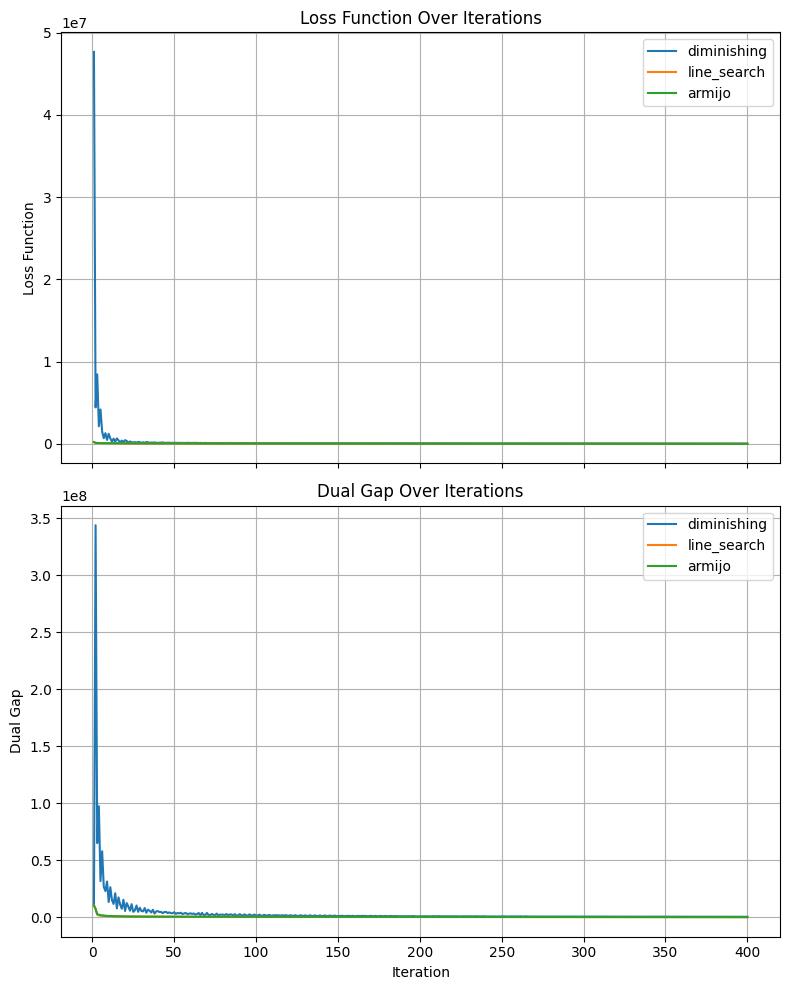
\includegraphics[height=0.75\textheight]{image/movielens_loss_gap_comparison}
        \hspace{0.5cm}
        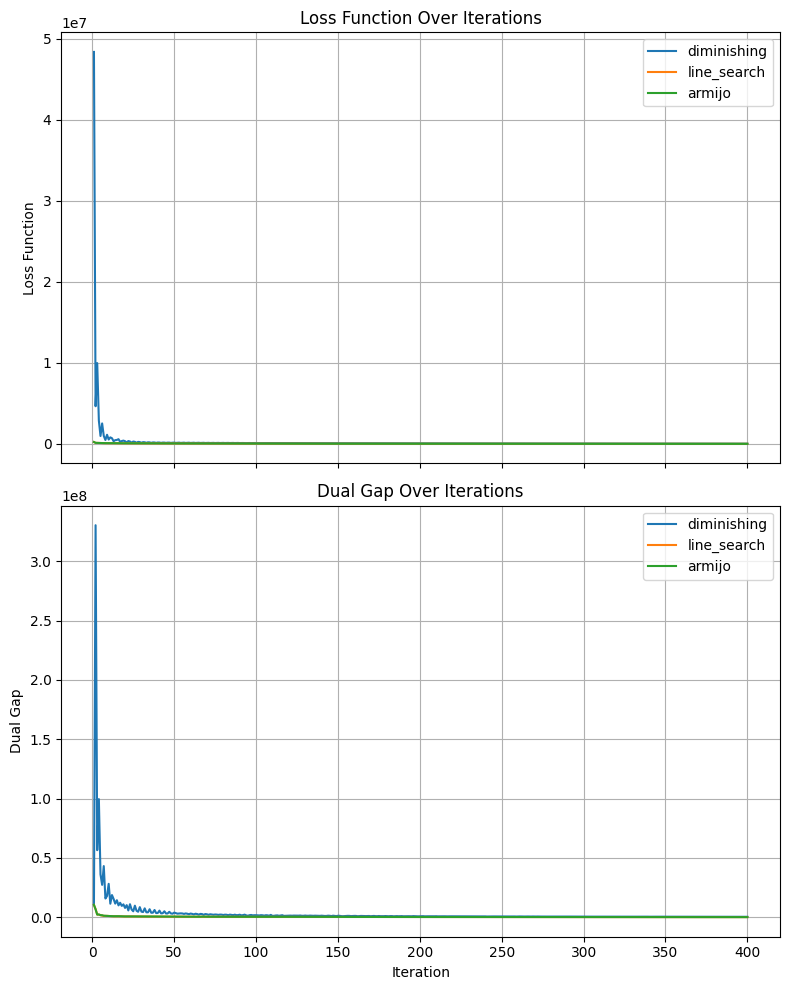
\includegraphics[height=0.75\textheight]{image/anime_loss_gap_comparison}
        \caption{Comparison of loss and dual gap for different \\
        step sizes. Left: MovieLens dataset. Right: Anime dataset.}
    \end{figure}
\end{frame}

\begin{frame}
    \frametitle{MovieLens}
    \vspace{-0.5cm}
    \begin{figure}[H]
        \centering
        \hspace{-0.55cm}
        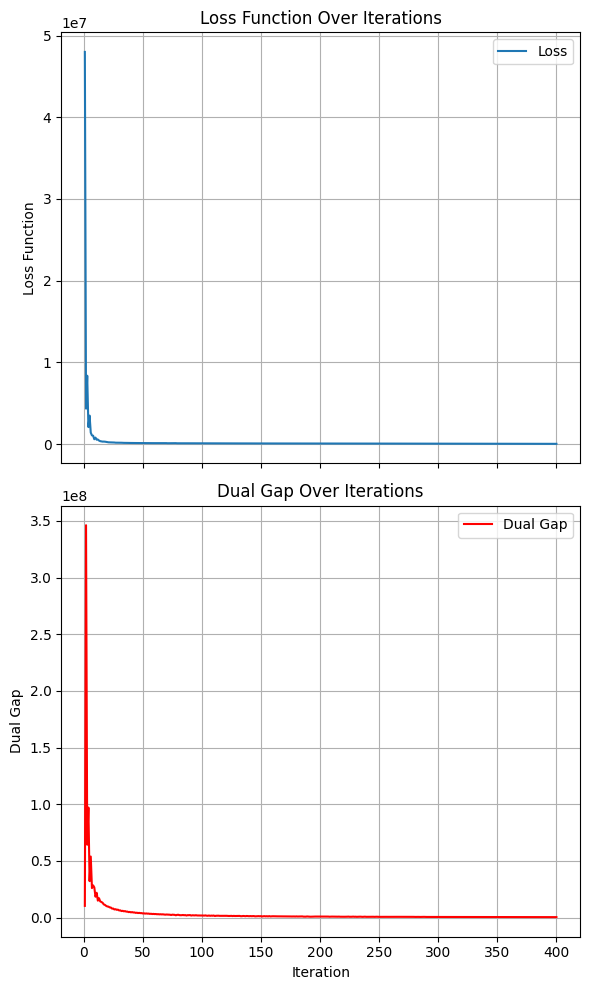
\includegraphics[height=0.75\textheight]{image/movielens_loss_gap_diminishing.png}
        \hspace{-0.2cm}
        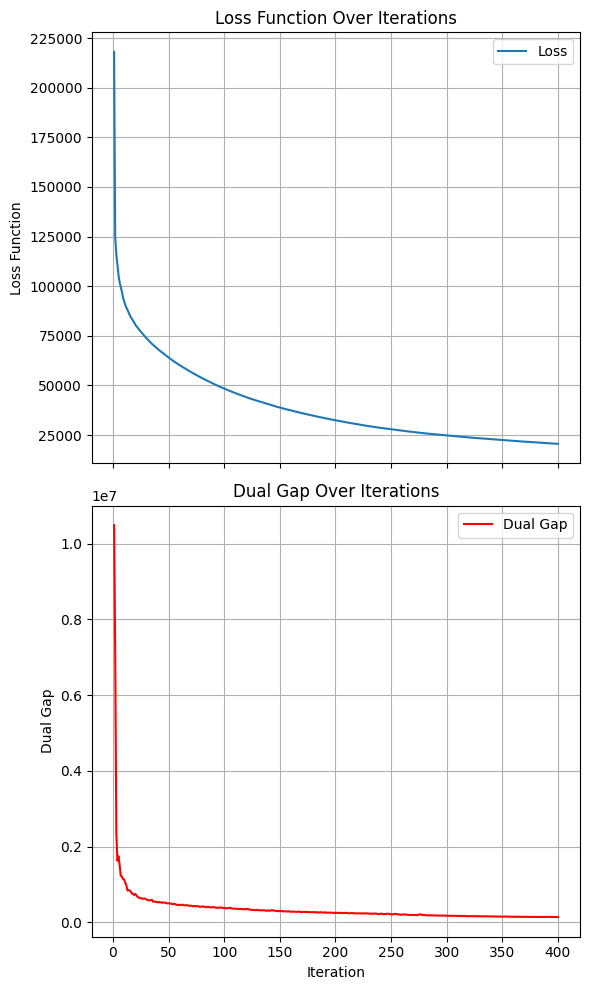
\includegraphics[height=0.75\textheight]{image/movielens_loss_gap_line_search.png}
        \hspace{-0.2cm}
        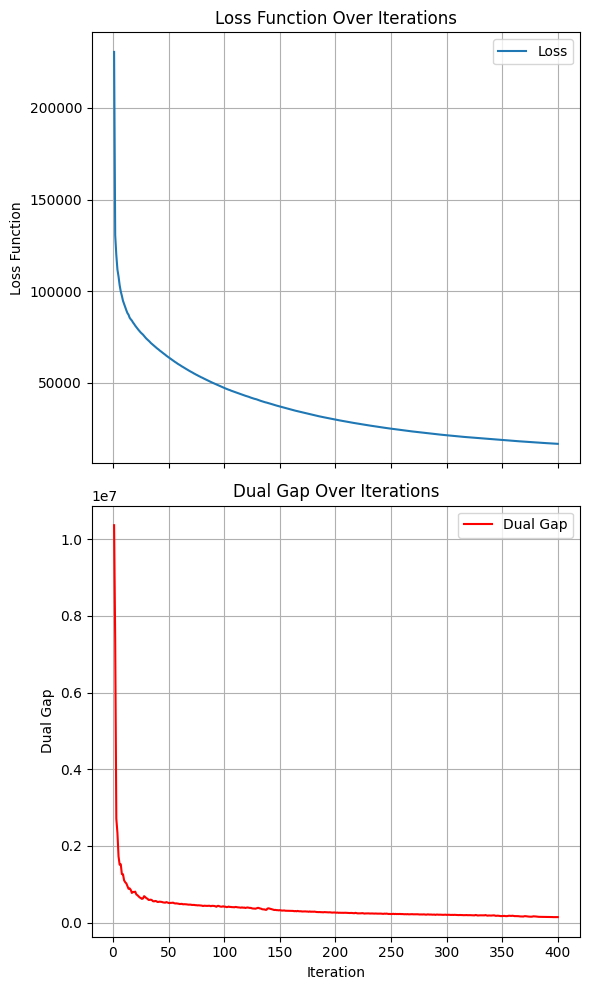
\includegraphics[height=0.75\textheight]{image/movielens_loss_gap_armijo.png}
        \caption{MovieLens dataset with different step size \\
        strategies: Diminishing, Exact Line Search, and Armijo Rule.}
    \end{figure}
\end{frame}

\begin{frame}
    \frametitle{Anime}
    \vspace{-0.5cm}
    \begin{figure}[H]
        \centering
        \hspace{-0.55cm}
        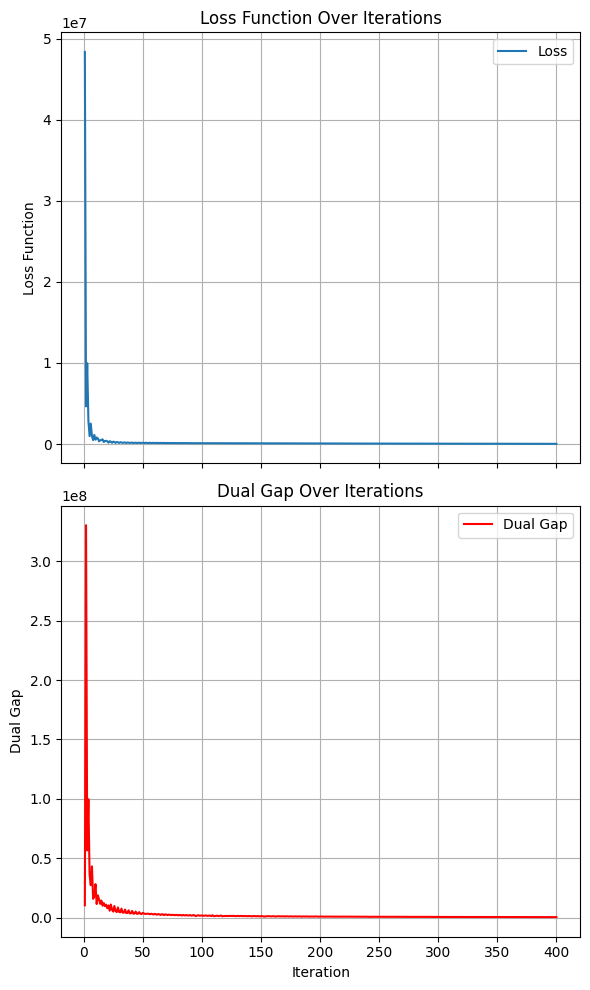
\includegraphics[height=0.75\textheight]{image/anime_loss_gap_diminishing.png}
        \hspace{-0.2cm}
        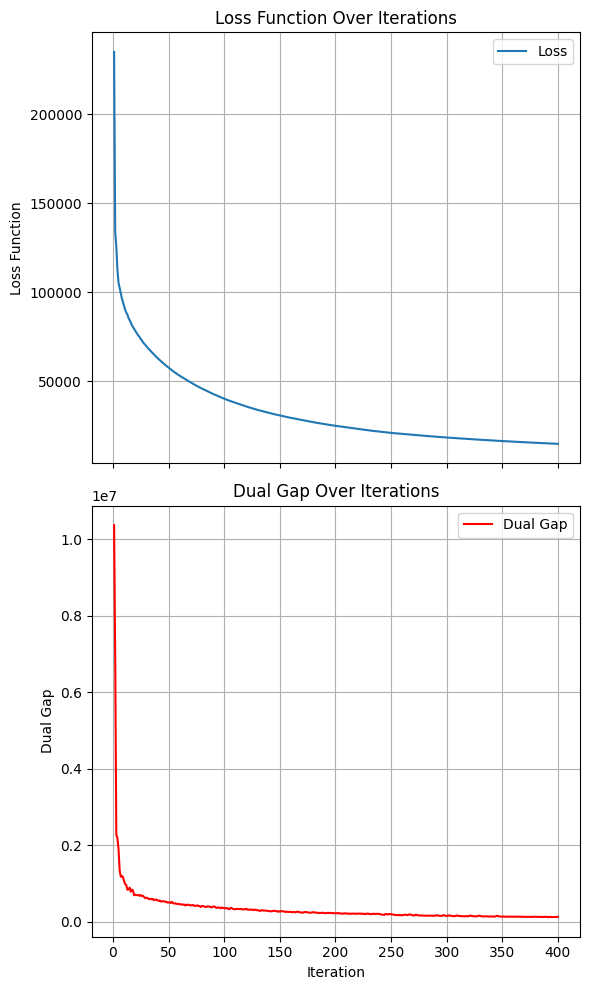
\includegraphics[height=0.75\textheight]{image/anime_loss_gap_line_search.png}
        \hspace{-0.2cm}
        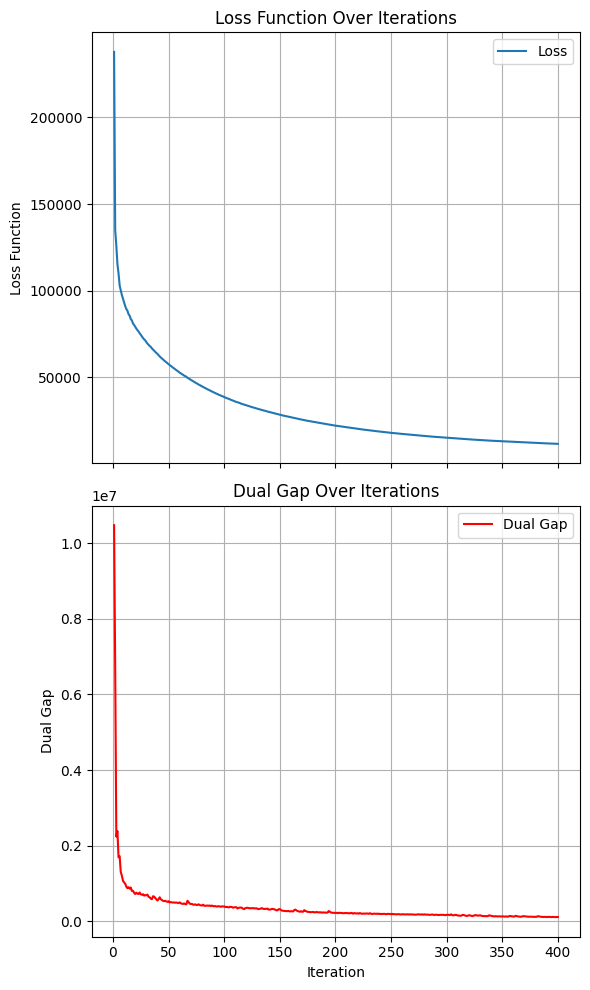
\includegraphics[height=0.75\textheight]{image/anime_loss_gap_armijo.png}
        \caption{Anime dataset with different step size \\
        strategies: Diminishing, Exact Line Search, and Armijo Rule.}
    \end{figure}
\end{frame}

\begin{frame}
    \frametitle{\textbf{Relative Accuracy Function and Results}}
     \vspace{-0.7cm}
    \textbf{Function Description:}
 The function computes the percentage of predictions (\( y_{\text{pred}} \)) that fall within a given \textbf{tolerance} of the true values (\( y_{\text{true}} \)).
 
     \vspace{0.3cm}
    \textbf{Results:}
    \begin{table}[H]
        \centering
        \begin{tabular}{|c|c|c|}
            \hline
            \textbf{Dataset} & \textbf{Step Size Strategy} & \textbf{Relative Accuracy (\%)} \\ \hline
            MovieLens & Diminishing & 62 \\ \hline
            MovieLens & Line Search & 82 \\ \hline
            MovieLens & Armijo & 88 \\ \hline
            Anime & Diminishing & 82 \\ \hline
            Anime & Line Search & 98 \\ \hline
            Anime & Armijo & 99 \\ \hline
        \end{tabular}
    \end{table}
\end{frame}



\end{document}